\chapter{Радосынь}

В этой главе, отдельно от всего, я предлагаю выяснить, что в летописи называли словом Радосынь.

Вопреки общепринятому мнению, по летописи нельзя вычислить, ни что такое Радосынь, ни где именно она находится.

Ипатьевская летопись, в 1111 (6618) году дополняет описание странного явления, о коем поведала за год 1110-й, 11 февраля:

\begin{quotation}
Се бо ангел вложи в сердце Володимеру Манамаху пустити братью свою на иноплеменникы, Русьскии князи; се бо, якоже рекохом, видинье видиша в Печерьском манастыри, еже стояше столп огнен на тряпезници, таже преступе на церковь и оттуда к Городцю; ту бо бяше Володимер в Радосыни, и тогда се ангел вложи Володимеру в сердце, нача понужа, якоже рекохом\footnote{Ангел побудил Владимира Мономаха вступить в бой с Половцами на реке Салнице. Ангел помогал в сражении – противника разил невидимый союзник Мономаха: «и падаху Половци пред полком Володимеровым, невидимо бьеми ангелом, яко се видяху мнози человеци, и главы летяху невидимо стинаемы на землю». Половцы рассказывали после победителям: «а друзии ездяху верху вас в оружьи светле и страшни, иже помогаху вам».}.
\end{quotation}

Отсюда следует, что когда Владимир Мономах был в Радосыни, от Лавры к Городку пошел огненный столп. В это время-то ангел и надоумил Владимира «пустити братью свою на иноплеменникы». А поелику «ту бо бяше» сказано после Городка, то Городок и Радосынь находятся в одном месте или рядом. Рядом, ежели Радосынь это селение. Но более вероятна трактовка – Городец стоял на водоеме либо местности Радосыни. Как это прояснить?

На карте РККА начала 1930-х годов я нашел ответ:

\begin{center}
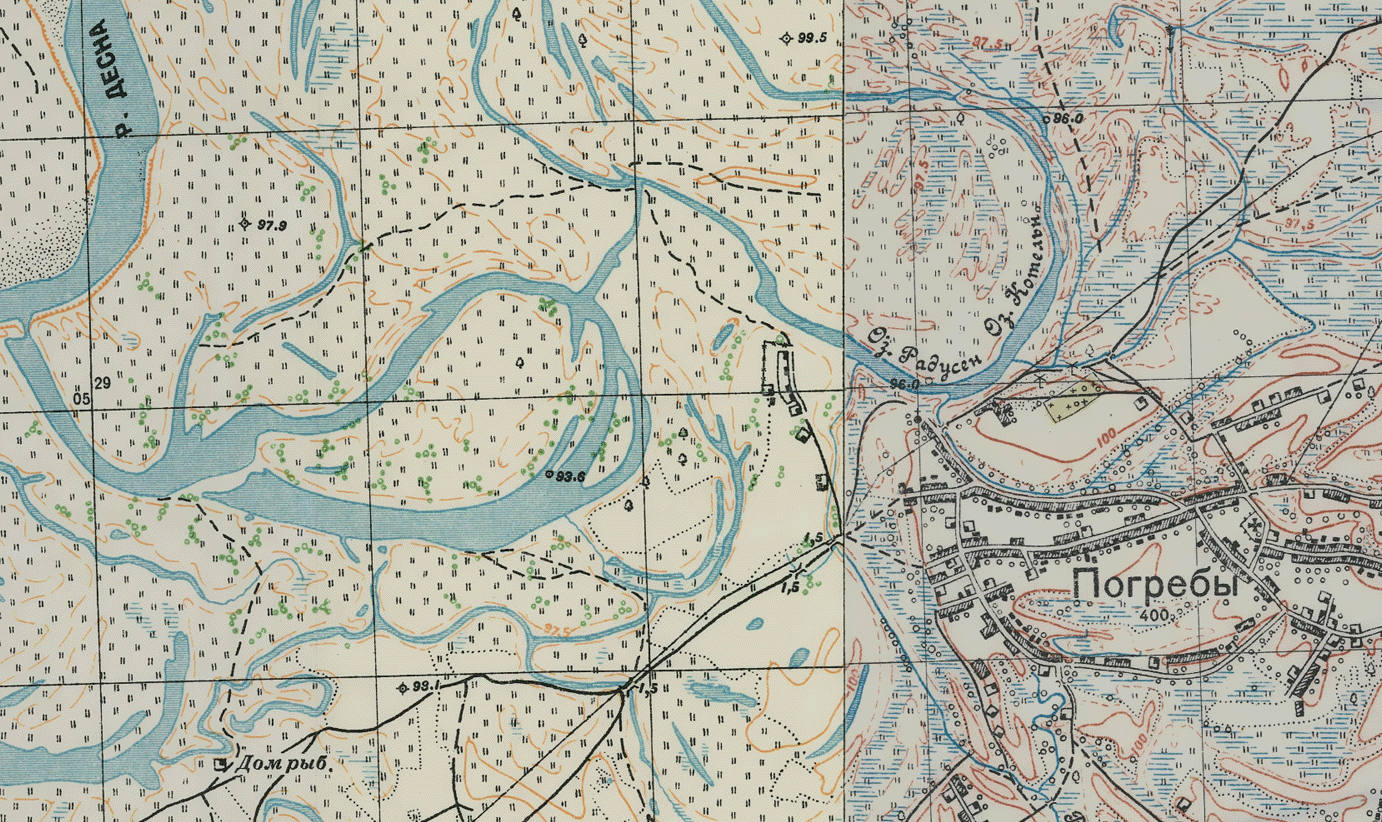
\includegraphics[width=\linewidth]{chast-gorodki/radosyn/radosen-big.jpg}
\end{center}

На тогдашней северо-западной окраине села Погребы, что находится к северо-западу от жилмассива Вигуро\-вщина-Троещина, мы видим «оз. Радусен»\footnote{50°33'35"N 
30°37'40"E}, переходящее в «оз. Котельн», причем оба по виду составляют старицу Десны.

Нынче южный берег Радусени обжит, вдоль него проходит улица Суворова, от перекрестков с улицей Кутузова (на западе\footnote{50°33'37"N  30°37'18"E}) и Европейской (на востоке\footnote{50°33'27"N 30°37'44"E}).

«Озеро Радусен», уже без подписи «оз. Котельн» рядом, показано и на карте РККА 1941 года.

Пожалуй, это снимает вопрос насчет географического положения летописной Радосыни. А Городец из той же записи за 1110 год если не погребен под усадьбами Погребов, то лежит где-то в окрестностях. Я бы поставил его на холме, где сейчас стоит шестая ТЭЦ. Видно не зря эта цепь возвышенностей именовалась Сторожевыми горами. Оттуда хорошо на северо-запад просматривается вся равнина с Погребами и Десной за ними. А с юго-запада эти горы омывало болото, бывшее прежде древним руслом Десны. Шальная мысль – а если не таким уж древним, и вовсе не болото протекало мимо Сторожевых гор?

Более общая картина, чтобы вы соотнесли, где Десна, Погребы, Троещина, Выгуровщина и Воскресенка:

\begin{center}
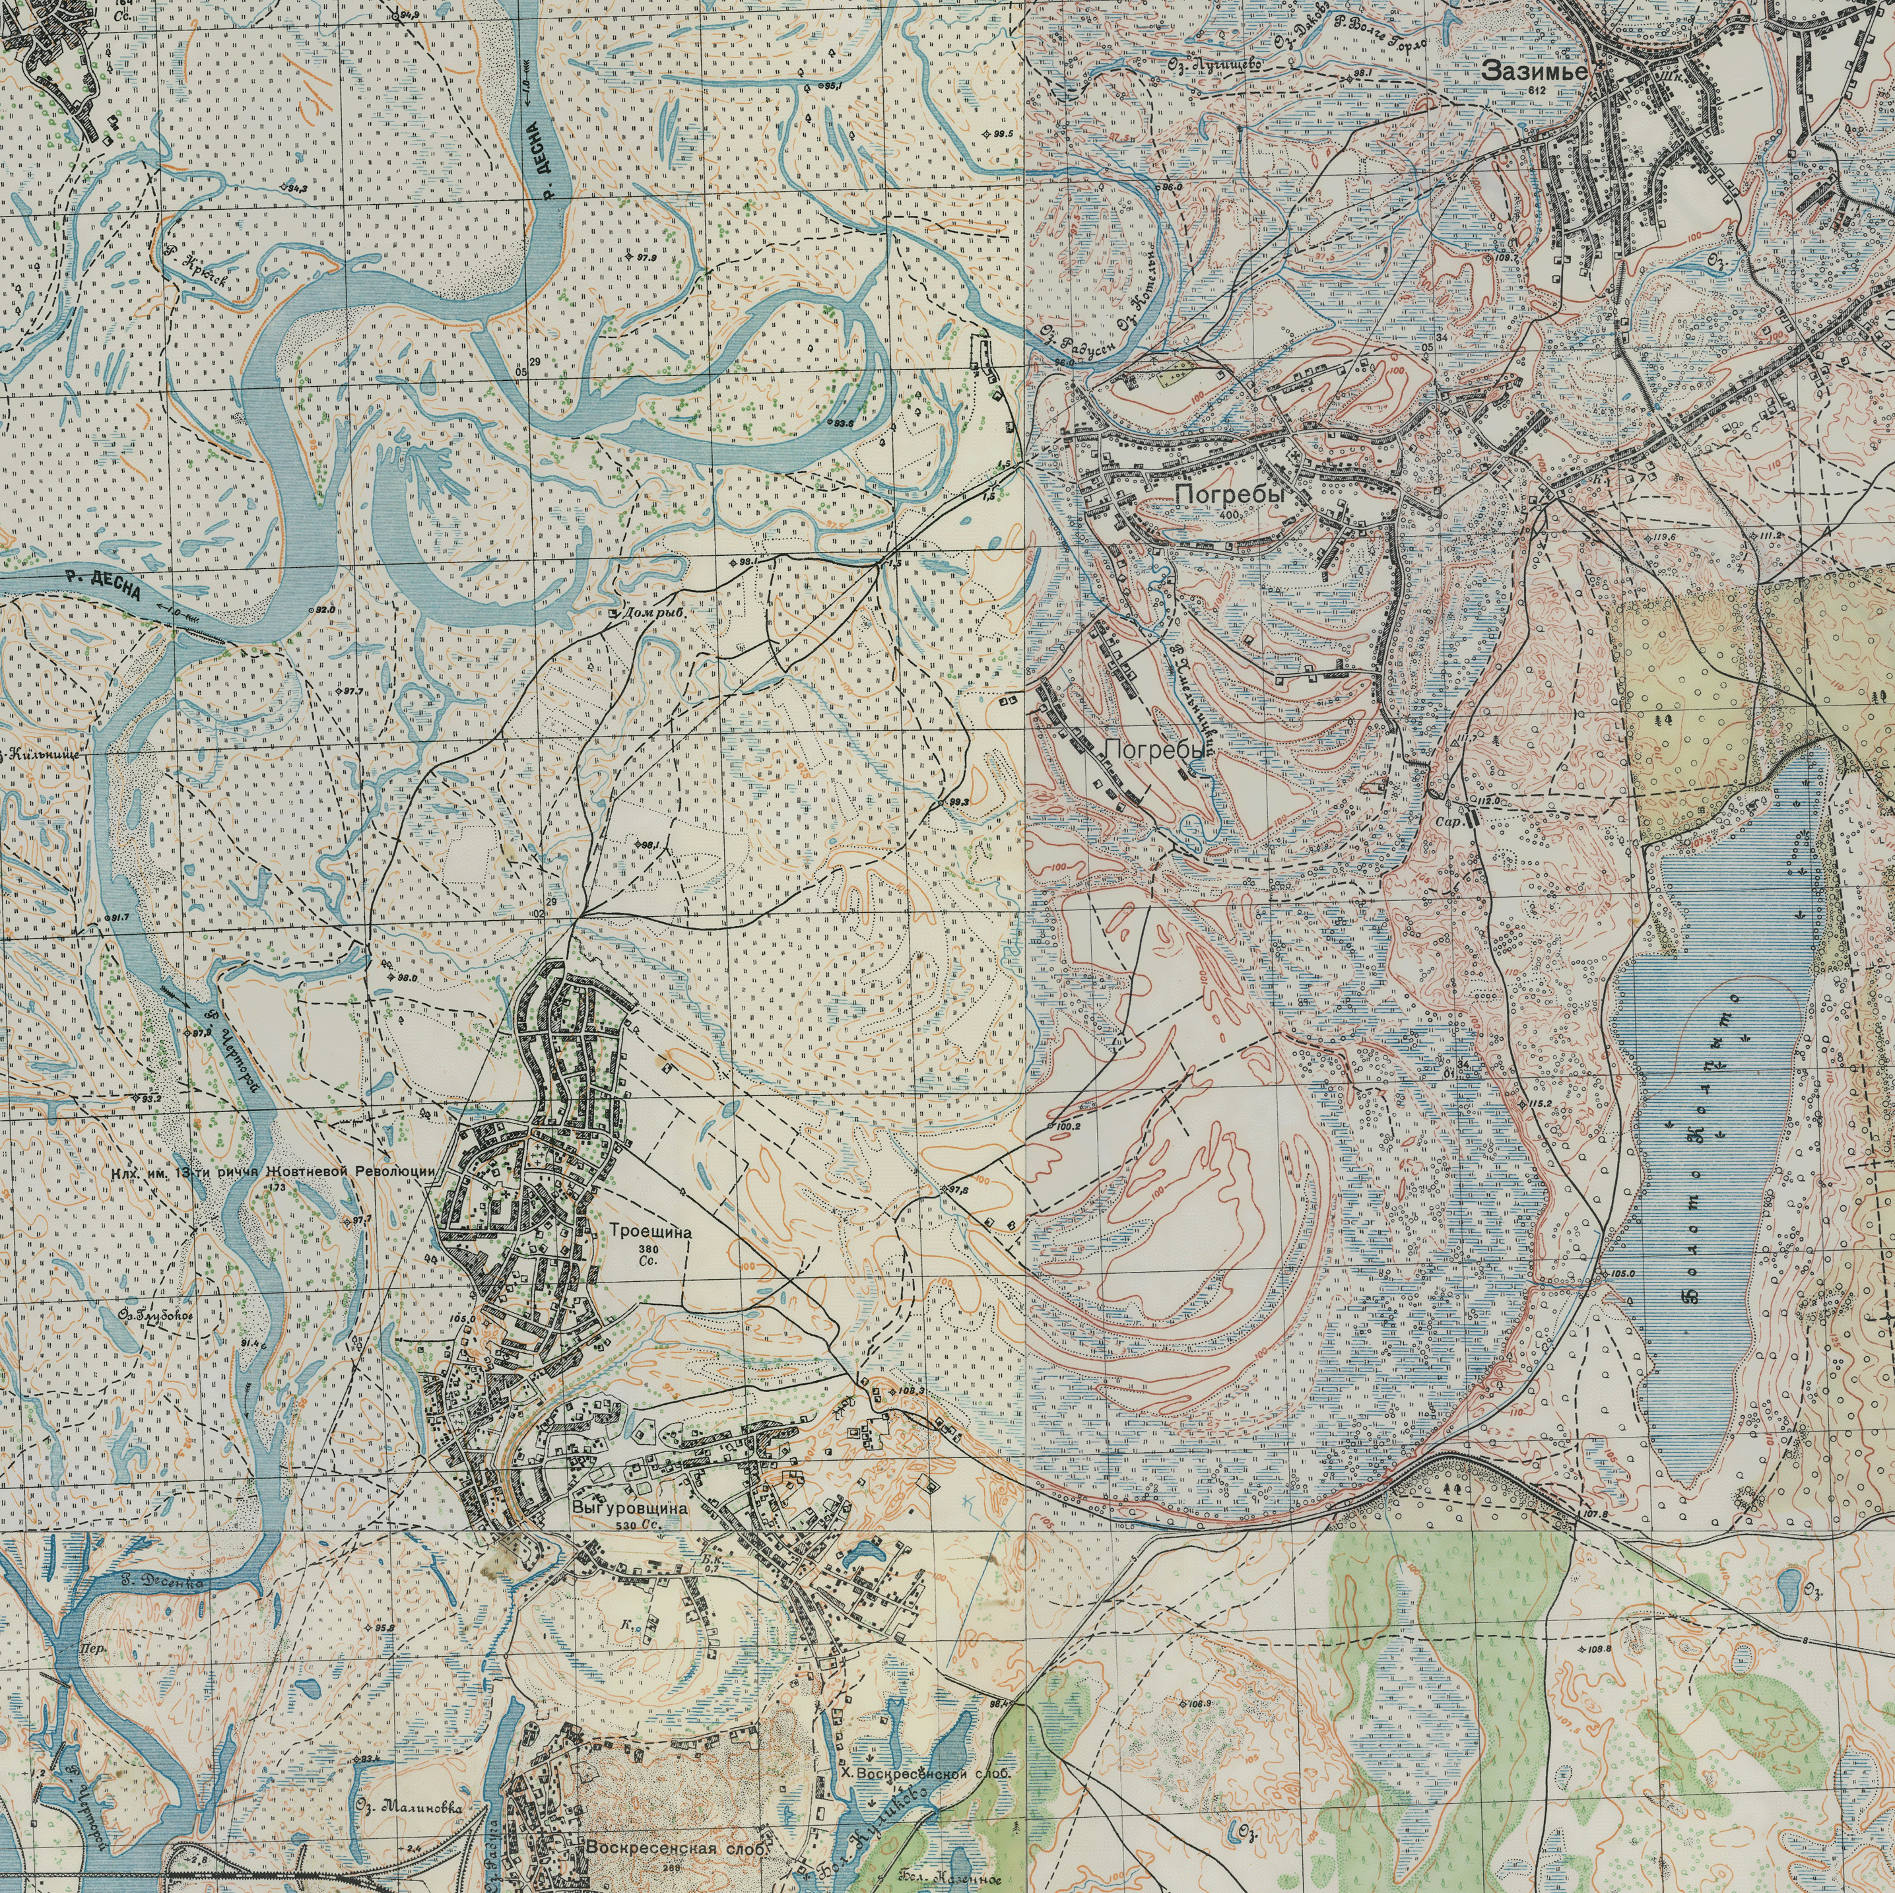
\includegraphics[width=\linewidth]{chast-gorodki/radosyn/radosen-s.jpg}
\end{center}

Итак, Радосынь была возле Погребов. На тридцатые годы 20 века искаженным именем Радосыни называлась старица Десны или остатки какой-то другой речки, в коих недостатка нет.

Но когда исказилось имя? Уже после выхода четвертой редакции «Ереси», где я впервые написал о Радосыни у Погребов, мне в руки попала любопытная подробная карта Киева и окрестностей, изданная в 1918 году при Скоропадском и основанная на съемке царского еще времени, 1897 года. Все названия на карте, которые поддавались переводу, были переведены на украинский – Николаи стали Миколаями, а Кадетская роща почему-то Кадетьскою Дібровою, хотя надо было бы Гаєм. При этом часть урочищ сохранили написание именно с русскоязычной карты – например Колпит вместо Ковпыта.

Как же обозначен на этой карте водоем, известный на карте РККА как «оз. Радусен»? А вот – «оз. Радусень».

\begin{center}
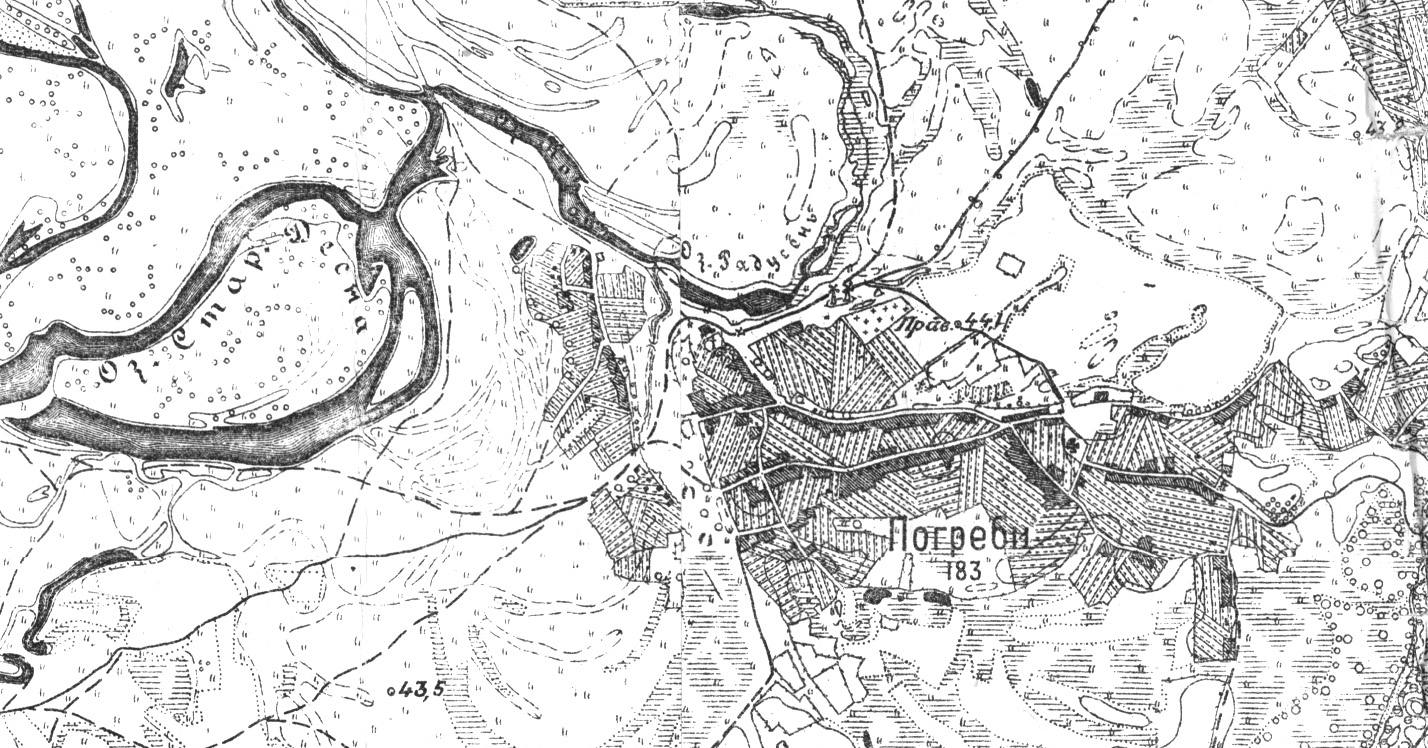
\includegraphics[width=\linewidth]{chast-gorodki/radosyn/rad-1918.jpg}
\end{center}

Это означает не только добавление мягкого знака и приближение к летописному звучанию (конечно, если мягкий знак не был внесен переводчиком), но и более раннее, на тридцать лет, упоминание «Радусени» в связи с этим водоемом!

Отличия между картой съемки 1897 и середины 1930-х не исчерпываются мягким знаком. На карте 1897 года западная часть водоема имеет некую подпись, которую я разобрать не могу. А вот часть, где потом подписано «оз. Котельн», на карте 1897 года относится к «Радусени»\footnote{Примечательно, как изменились названия соседствующих к северу озер за 30 лет. Привожу попарно названия с карты 1918 и РККА. «Лучисте» – «Лучищево», «Забок» – «Дяковэ», «Козарка» – «Козарка», «Козарка Довга» – «Громадская Козарка», впрочем последняя сильно изменилась, перегороженная гатью, и западная часть «Козарки довгой» занято на карте РККА уже ручьем или речкой Резовахой.}.  

Считаю, что в 1110 году Радосынь находилась там же, однако чем она была – местностью, по имени которой назвали водоем? Только водоемом? Может, там был исток речки Радунки и ее русло оттуда тянулось до Выгуровщины и южнее?

К остаткам «озера Радусен» я попал летом 2012 года, когда еще не знал, что это такое. Ездил на велике купаться на Десну и проезжал мимо. Слева были дома, справа поле и в нем старица, заросшая кувшинками. Она переходила в какие-то пересохшие иловые поля, разделенные на участки, что продавались оптом и в розницу.

Спустя несколько лет в воде появился земснаряд, старицу на западной трети принялись углублять, намывая берега для строительства. Еще одно летописное урочище стало застраиваться.
\vspace*{\fill}
\begin{center}
\includegraphics[width=\linewidth]{chast-gorodki/radosyn/\myimgprefix DSC_0014.jpg}

\textit{Снимок 2012 года.}
\end{center}
\vspace*{\fill}

\newpage
\vspace*{\fill}
\begin{center}
\includegraphics[width=\linewidth]{chast-gorodki/radosyn/\myimgprefix IMG_20130612_171938.jpg}
\end{center}

\begin{center}
\includegraphics[width=\linewidth]{chast-gorodki/radosyn/\myimgprefix IMG_20130612_171940.jpg}
\textit{Снимки 2013 года.}
\end{center}
\vspace*{\fill}
\newpage


Названия «Радусен» и «Котелн». Первое со спокойной совестью сопоставимо с Радосынью. Больше «Радосынь» нигде не упоминается, только единожды в летописи. В произношении «Радусен» и смежным «Котелн» чувствуется что-то иностранное, немецкое. На современных картах «Радусен» опускают, а пишут «Котельня».

О селе Погребы Броварского района (есть еще одноименное Васильковского). Оно находится в низине между Сторожевым горами, на которых стоит ТЭЦ-6, и Десной. Из статьи в статью кочуют сведения без ссылки на источник, что в Погребах археологи нашли «печать Ратибора», тысячника и печатника Владимира Мономаха. А в 1956 году – печать на греческом языке, князя Андрея Боголюбского.

Среди других находок археологов – кремневые орудия, трипольская фигурка, бронзовые скифские фигурки и наконечники стрел, амфоры, римские монеты.

В урочищах Келийки и Поломы есть курганы, которых относят к зарубинецкой культуре – я впрочем их не видел.

Из разных источников узнаю много любопытного про это село. Что лежало оно на давней Дуковой дороге. А ведь «дюк» это князь.

Названия окрестных урочищ – речка Кодачок, Боженька\footnote{Вероятно тут: 50°33'36"N  30°34'57"E, где от Десны на восток идет большая петлеобразная старица.}, Завборок, Бруева долина, Тенетница, Мижудит, Пасека, Ланы, Праторев, Кайки, Роги, Выгуровская дубрава, Ланы, Остров, Старое село, Залющики (заливаются Десной в половодье), Терник, Клуница (поле к северу от 20 микрорайона Вигуровщины-Троещины), Витовская (поле к северу от 20 и 13 микрорайонов). Выгоны: Поддубное, Майдан (западная окраина села\footnote{50°32'59"N 30°37'43"E}), Остров, Великий лес, Прогний, Завирком. Луки: Закодачче, Роги, Плавни, Запрериз, Застарушка, Заозера, Задесенье, Высокое.

На 1784 год село входило в состав Киевской казачьей сотни, насчитывало 30 дворов и 103 души.

1858 год – 90 дворов, 495 казенных крестьян. 1897 двора, 1117 душ. 1925 – 318 дворов, 1700 жителей.

%В 1896 году была построена церковь Успения Богородицы.

В Погребах было записано предание о болоте Ковпыт:

\begin{quotation}
Колись було село, і воно завалилось в болото, а щоб воно вийшло нагору, треба тричі верхи об'їхать навколо нього на Великдень. Один чоловік і об'їхав. І стало видно і село, і люди. Але кінь впав, і все пропало, знов провалилось село.
\end{quotation}

Напоминает чем-то рассказы о жилищах эльфов, о граде Китеже, о невидимом дворце княгини Ольги в Выбутах.

Также я где-то читал, что в Ковпыте еще по 1960-е можно было наблюдать торчащую наружу верхушку церковного купола – остатки утонувшего села.

Про Городок же отмечу еще одну странность, которая часто проявляется при упоминаниях о Городке. Не сказано, что Мономах был в Городке. Сказано, что он был в Радосыни. Заметим это. Не в Городке.

История про чудесное явление с огненным столпом, что отправился от Лавры к Городку, в записи за 1110 год рассказана иначе, без Мономаха, Радосыни и Городка – кажется, мы имеем дело с двумя источниками, светским (за 1111 год) и духовным 1110 года:

\begin{quotation}
бысть знамение в Печерьском манастыри, февраля в 11 день: явися столп огнен от земля до небесе, а молнья осветиша всю землю, и на небеси погреме в час 1 нощи; весь мир виде. 

Сесь же столп ста на тряпезници камяней, яко не видити хреста бяше, и стоя мало, ступи на церковь и ста над гробом Федосьевом и потом над верх съступи, аки ко въстоку лицем, и потом невдимо бысть.

Се же бяше не огнь, ни столп, но вид ангельский: ангел бо сице является, ово столпом огненом, ово же пламененом; якоже же рче Давид: творя ангелы своя духы и слугы своя огнь пламян;
\end{quotation}
